\documentclass[13pt,a4paper]{article}
\usepackage[utf8]{inputenc}
\usepackage[T5]{fontenc}
\usepackage[vietnamese]{babel}
\usepackage{amsmath, amsfonts, amssymb}
\usepackage{graphicx}
\usepackage{booktabs}
\usepackage{hyperref}
\usepackage{listings}
\usepackage{color}
\usepackage{geometry}
\usepackage{setspace}
\usepackage{titlesec}
\usepackage{caption}
\usepackage{indentfirst}
\usepackage{algorithm}
\usepackage{algpseudocode}
\usepackage{needspace}

% --- Cấu hình lề chuẩn VNU-UET ---
\geometry{
    a4paper,
    top=2.5cm,
    bottom=3.0cm,
    left=3.0cm,
    right=2.0cm
}

\setstretch{1.3} 
\setlength{\parindent}{1cm} 
\setlength{\parskip}{6pt}
\raggedbottom 

\usepackage{fancyhdr}
\pagestyle{fancy}
\fancyhf{}
\fancyfoot[C]{\thepage} 
\renewcommand{\headrulewidth}{0pt}

\titleformat{\section}{\normalfont\Large\bfseries}{Chương \thesection.}{0.5em}{}
\titleformat{\subsection}{\normalfont\large\bfseries}{\thesubsection.}{0.5em}{}
\titleformat{\subsubsection}{\normalfont\normalsize\bfseries}{\thesubsubsection.}{0.5em}{}

\captionsetup[table]{position=above, skip=5pt}
\captionsetup[figure]{position=below, skip=5pt}

\definecolor{backcolour}{rgb}{0.97,0.97,0.97}
\definecolor{codegreen}{rgb}{0,0.6,0}
\definecolor{codepurple}{rgb}{0.58,0,0.82}
\definecolor{codeblue}{rgb}{0.13,0.13,1}

\lstset{
    backgroundcolor=\color{backcolour},   
    basicstyle=\ttfamily\small,
    commentstyle=\color{codegreen},
    keywordstyle=\color{codeblue}\bfseries,
    stringstyle=\color{codepurple},
    breaklines=true,
    frame=single,
    numbers=left,
    numberstyle=\tiny\color{gray},
    tabsize=4,
    showstringspaces=false
}

\begin{document}

% --- TRANG TRẮNG ĐỂ CHỜ THÊM BÌA ---
\mbox{}
\newpage

% --- MỤC LỤC ---
\newpage
\tableofcontents
\newpage

\pagenumbering{arabic}

% ================= CHƯƠNG 1 =================
\section{Mở đầu}

\subsection{Tính cấp thiết của đề tài}
Trí tuệ nhân tạo trong trò chơi đối kháng (Adversarial Search) là một lĩnh vực nghiên cứu nền tảng của Khoa học Máy tính. Các trò chơi board game như cờ vua, cờ vây, hay cờ Caro thường sở hữu một không gian trạng thái vô cùng lớn. Việc giải quyết các bài toán này không chỉ chứng minh khả năng tính toán của máy móc mà còn giúp chúng ta khám phá ra các thuật toán tìm kiếm và tối ưu hóa ưu việt. Đề tài "Xây dựng AI chơi cờ Caro 9x9" là một cơ hội tuyệt vời để sinh viên vận dụng lý thuyết cây trò chơi (Game Tree) vào thực tiễn lập trình, qua đó rèn luyện tư duy thiết kế cấu trúc dữ liệu và tối ưu hiệu năng phần mềm.

\subsection{Mục tiêu và Phạm vi nghiên cứu}
Đồ án đặt ra mục tiêu xây dựng một tác tử AI hoàn chỉnh có thể thi đấu công bằng với con người theo đúng luật cờ Caro hiện đại. Hệ thống phải đảm bảo:
\begin{itemize}
    \item \textbf{Độ chính xác:} Tính toán và đưa ra nước đi hợp lệ, không vi phạm luật chơi.
    \item \textbf{Độ thông minh:} Khả năng phản xạ chặn các nước cờ nguy hiểm và biết cách thiết lập bẫy tấn công.
    \item \textbf{Hiệu suất thực thi:} Trả về kết quả trong thời gian giới hạn (dưới 2 giây/lượt) bằng cách ứng dụng Alpha-Beta Pruning.
\end{itemize}

% ================= CHƯƠNG 2 =================
\section{Cơ sở lý thuyết}

\subsection{Mô tả bài toán cờ Caro}
Trò chơi cờ Caro diễn ra trên một mạng lưới lưới tọa độ Descartes $9 \times 9$. Gọi trạng thái hiện tại của bàn cờ là $S$, tập hợp tất cả các nước đi hợp lệ từ trạng thái $S$ là $Actions(S)$. Hàm chuyển đổi trạng thái $Result(S, a)$ sẽ trả về một trạng thái $S'$ mới sau khi áp dụng nước đi $a \in Actions(S)$. Bài toán yêu cầu tìm kiếm chuỗi hành động tối ưu để đạt đến trạng thái kết thúc (Terminal State) có lợi nhất.

\subsection{Luật chơi và điều kiện thắng}
Để chuẩn hóa đầu vào cho AI, luật chơi được định nghĩa bằng các hằng số và nguyên lý toán học như sau:
\begin{itemize}
    \item \textbf{Ký hiệu:} Người chơi là \texttt{1} (X), Máy tính là \texttt{2} (O), ô trống là \texttt{0} (.).
    \item \textbf{Điều kiện thắng:} Một trạng thái $S$ được coi là chiến thắng cho người chơi $P$ nếu tồn tại ít nhất 4 tọa độ liên tiếp $(r_i, c_i)$ theo cùng một vectơ hướng $\vec{v} \in \{(1,0), (0,1), (1,1), (1,-1)\}$ sao cho $S(r_i, c_i) = P$ với mọi $i \in [1, 4]$.
    \item \textbf{Không chặn hai đầu:} Việc hai đầu của chuỗi 4 quân bị đối phương chặn không làm mất đi tính chiến thắng.
\end{itemize}

\begin{figure}[h]
    \centering
    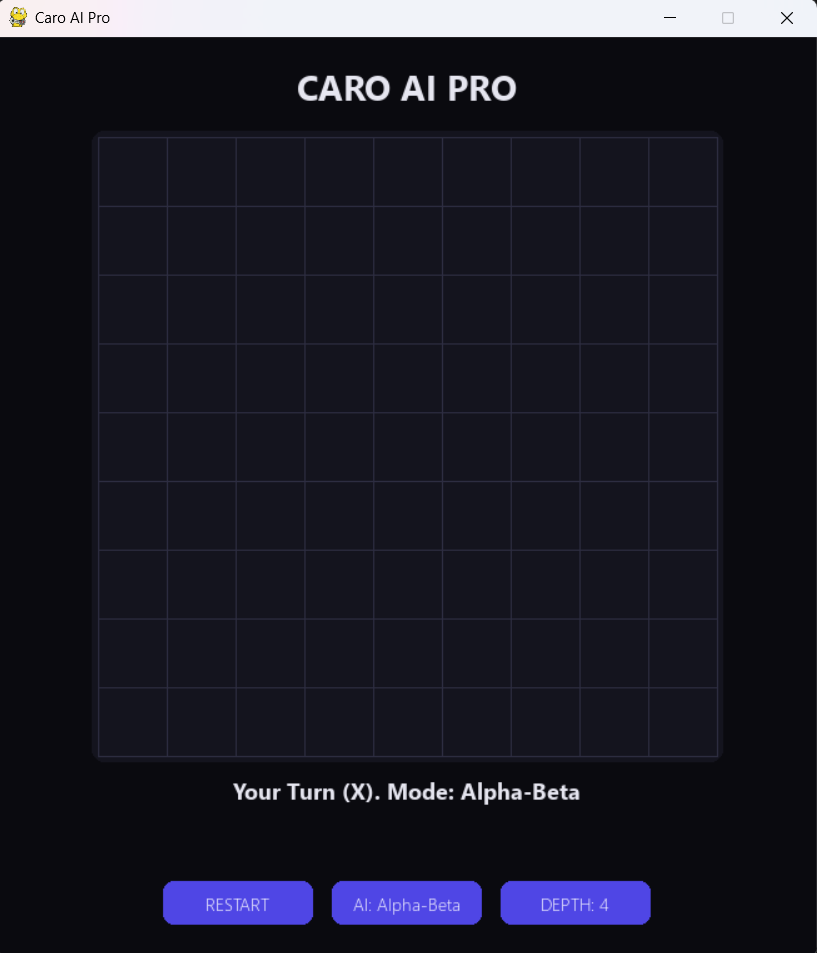
\includegraphics[width=0.6\textwidth]{image/A.png}
    \caption{Giao diện bàn cờ trống ở trạng thái khởi tạo}
    \label{fig:board_init}
\end{figure}

\subsection{Thuật toán Minimax}
Thuật toán Minimax là nền tảng của trí tuệ nhân tạo trong các trò chơi đối kháng có tổng bằng không (zero-sum game). Thuật toán hoạt động dựa trên nguyên lý: người chơi MAX (máy tính) luôn cố gắng tối đa hóa điểm số, trong khi người chơi MIN (đối thủ) luôn cố gắng tối thiểu hóa điểm số đó. Quá trình tìm kiếm tạo ra một cây trò chơi, trong đó các nút đại diện cho các trạng thái của bàn cờ và các cạnh đại diện cho các nước đi.

Ta định nghĩa hàm giá trị $Minimax(S)$ tại trạng thái $S$ như sau:
\begin{itemize}
    \item $Minimax(S) = \text{Utility}(S)$ nếu $S$ là trạng thái lá (kết thúc) hoặc đạt tới độ sâu giới hạn ($Depth = 0$).
    \item $Minimax(S) = \max_{a \in Actions(S)} Minimax(Result(S, a))$ nếu đến lượt MAX.
    \item $Minimax(S) = \min_{a \in Actions(S)} Minimax(Result(S, a))$ nếu đến lượt MIN.
\end{itemize}

Độ phức tạp thời gian của thuật toán là $O(b^d)$ và độ phức tạp không gian là $O(bd)$, trong đó $b$ (branching factor) là số lượng nước đi hợp lệ trung bình tại mỗi bước, và $d$ là độ sâu tìm kiếm. Tuy nhiên, với bàn cờ cờ Caro $9 \times 9$, không gian trạng thái lên tới $3^{81}$, hệ số $b$ ở giai đoạn đầu có thể lên tới 81, khiến Minimax thuần túy chỉ có thể duyệt sâu từ 2 đến 3 tầng trong thời gian thực tế.

\subsection{Thuật toán Alpha-Beta Pruning}
Để khắc phục hạn chế về thời gian của Minimax, kỹ thuật cắt tỉa Alpha-Beta (Alpha-Beta Pruning) được áp dụng nhằm giảm thiểu số lượng nút cần đánh giá trên cây tìm kiếm mà vẫn đảm bảo kết quả không thay đổi. Thuật toán duy trì hai tham số truyền xuống trong quá trình đệ quy:
\begin{itemize}
    \item $\alpha$: Giá trị tốt nhất (cao nhất) mà MAX có thể đảm bảo đạt được dọc theo nhánh từ gốc đến nút hiện tại.
    \item $\beta$: Giá trị tốt nhất (thấp nhất) mà MIN có thể đảm bảo đạt được dọc theo nhánh từ gốc đến nút hiện tại.
\end{itemize}

\textbf{Cơ chế cắt tỉa:} Tại bất kỳ nút MIN nào, nếu giá trị tạm thời $v \le \alpha$, ta lập tức dừng việc xét các nhánh con còn lại của nút đó (vì MAX ở nút cha chắc chắn sẽ không chọn nhánh đi qua nút MIN này). Tương tự, tại bất kỳ nút MAX nào, nếu $v \ge \beta$, ta cũng cắt bỏ các nhánh con. Điều kiện cắt tỉa chung được phát biểu gọn là $\beta \le \alpha$.

Việc áp dụng Alpha-Beta giúp độ phức tạp thời gian giảm từ $O(b^d)$ xuống xấp xỉ $O(b^{d/2})$ trong trường hợp lý tưởng (khi các nước đi tốt nhất luôn được duyệt trước). Điều này cho phép AI nhân đôi độ sâu tìm kiếm trong cùng một khoảng thời gian so với Minimax thông thường.

% ================= CHƯƠNG 3 =================
\section{Phân tích thiết kế và Cài đặt hệ thống}

\subsection{Cách biểu diễn trạng thái bàn cờ}
Bàn cờ được cài đặt bằng đối tượng \texttt{Board} chứa một mảng hai chiều (List of Lists) trong Python.
\needspace{15\baselineskip}
\begin{lstlisting}[language=Python, caption=Khởi tạo mảng hai chiều biểu diễn bàn cờ]
class Board:
    def __init__(self, size=9):
        self.size = size
        # Khoi tao ma tran 9x9 voi gia tri 0 (ô trong)
        self.grid = [[0 for _ in range(size)] for _ in range(size)]
\end{lstlisting}
Cách tiếp cận này không chỉ dễ dàng thao tác mà còn cho phép tối ưu quá trình sao chép trạng thái (Deepcopy) phục vụ cho thuật toán đệ quy.

\subsection{Cách sinh nước đi hợp lệ và Tối ưu hóa}
Để giảm hệ số phân nhánh (Branching Factor), chương trình áp dụng kỹ thuật \textbf{Radius-2 Search}. Thay vì xem xét tất cả các ô trống, thuật toán chỉ trả về các ô nằm trong bán kính 2 ô vuông tính từ các quân cờ hiện tại.
\needspace{15\baselineskip}
\begin{lstlisting}[language=Python, caption=Cài đặt thuật toán sinh nước đi với Radius Search]
def get_valid_moves(self, search_radius=2):
    moves = set()
    # Tim tat ca cac quan co da danh tren ban
    pieces = [(r, c) for r in range(self.size) for c in range(self.size) 
              if self.grid[r][c] != 0]
              
    if not pieces: return [(self.size // 2, self.size // 2)] # Đanh tam

    # Phat trien theo ban kinh radius
    for r, c in pieces:
        for dr in range(-search_radius, search_radius + 1):
            for dc in range(-search_radius, search_radius + 1):
                nr, nc = r + dr, c + dc
                if 0 <= nr < self.size and 0 <= nc < self.size:
                    if self.grid[nr][nc] == 0:
                        moves.add((nr, nc))
    return list(moves)
\end{lstlisting}
Phương pháp này giúp giới hạn không gian trạng thái, loại bỏ các phép tính dư thừa ở vùng rìa bàn cờ và cải thiện đáng kể thời gian duyệt cây.

\subsection{Thuật toán Minimax đã cài đặt}
Thuật toán Minimax được nhóm cài đặt thông qua hàm đệ quy \texttt{minimax\_search(board, depth, is\_maximizing)}. Ở mỗi bước, hàm sẽ kiểm tra điều kiện dừng: nếu trò chơi kết thúc (có người thắng/hòa) hoặc đạt \texttt{depth == 0}, hàm sẽ gọi \texttt{Evaluator.evaluate()} để trả về điểm tĩnh của bàn cờ hiện tại. Nếu chưa dừng, hàm tiếp tục gọi \texttt{get\_valid\_moves()} để lấy danh sách các ô có thể đánh. Tuy nhiên, ở môi trường Caro thực tế, Minimax cài đặt cơ bản bộc lộ tốc độ cực kỳ chậm, không thể vượt qua độ sâu 3.

\subsection{Thuật toán Alpha-Beta đã cài đặt}
Để tối ưu hóa, thuật toán cắt tỉa Alpha-Beta được cài đặt hoàn thiện trong hàm \texttt{alpha\_beta\_search(board, depth, alpha, beta, is\_maximizing)}. Điểm nổi bật trong mã nguồn là việc tích hợp cơ chế cập nhật $\alpha$, $\beta$ và ngắt vòng lặp (break) ngay khi phát hiện nhánh vô ích:

\needspace{15\baselineskip}
\begin{lstlisting}[language=Python, caption=Cơ chế cắt tỉa và lưu Flag trong hàm Alpha-Beta]
if is_maximizing:
    max_val = -float('inf')
    for r, c in valid_moves[:30]:
        board.make_move(r, c, self.ai_player)
        val, _ = self.alpha_beta_search(board, depth - 1, alpha, beta, False)
        board.undo_move(r, c, self.ai_player)
        
        if val > max_val:
            max_val = val
            best_move = (r, c)
        alpha = max(alpha, val)
        if beta <= alpha: break
        
    flag = 0 # EXACT
    if max_val <= orig_alpha: flag = 2 # UPPER
    elif max_val >= orig_beta: flag = 1 # LOWER
    self.memo[state_key] = (max_val, depth, flag, best_move)
    return max_val, best_move
\end{lstlisting}

Ngoài ra, thay vì copy toàn bộ bàn cờ (\texttt{deepcopy}) vốn rất tốn kém tài nguyên ở mỗi bước sinh nhánh con, nhóm sử dụng kỹ thuật "Đánh thử và Hoàn tác" (\texttt{make\_move} sau đó \texttt{undo\_move}). Kỹ thuật này giúp giải phóng bộ nhớ và tăng tốc độ duyệt nhánh lên nhiều lần, hỗ trợ trực tiếp cho khả năng cắt nhánh sâu của Alpha-Beta.

\subsection{Kỹ thuật Iterative Deepening}
Để đảm bảo AI luôn trả về kết quả trong thời gian thực (ví dụ 2 giây), nhóm áp dụng \textbf{Iterative Deepening} (Tìm kiếm sâu dần). Thuật toán không duyệt thẳng vào độ sâu $D$, mà sẽ duyệt từ $d=1$ tăng dần đến $D$.
\needspace{15\baselineskip}
\begin{lstlisting}[language=Python, caption=Cài đặt Iterative Deepening với giới hạn thời gian]
for current_depth in range(1, max_depth + 1):
    score, move = self.alpha_beta_search(board, current_depth, -float('inf'), float('inf'), True)
    if move:
        best_move = move
    
    # Nhanh chong dung viec tim kiem neu vuot qua 2 giay
    if time.time() - start_time > 2.0:
        break
\end{lstlisting}
Kỹ thuật này đảm bảo hệ thống luôn lưu trữ kết quả tốt nhất ở độ sâu trước đó, cho phép phản hồi kịp thời nước đi ưu ưu nhất khi đạt giới hạn thời gian quy định.

\subsection{Kỹ thuật Transposition Table (Bộ nhớ đệm)}
Trong cờ Caro, một trạng thái bàn cờ có thể được tạo ra từ nhiều trình tự đánh khác nhau (đảo thứ tự nước đi). Để tránh việc Minimax phải tính lại các trạng thái đã biết, nhóm sử dụng \textbf{Transposition Table} bằng cấu trúc Dictionary của Python. Khóa hash được tạo siêu tốc thông qua \texttt{str(board.grid)} kết hợp với việc kiểm tra các cờ toán học (EXACT, LOWER, UPPER) thay vì chỉ lưu một giá trị đại diện dễ gây sai số.
\needspace{15\baselineskip}
\begin{lstlisting}[language=Python, caption=Cài đặt Transposition Table luu tru ket qua]
state_key = (str(board.grid), is_maximizing)

if state_key in self.memo:
    val, d, flag, m = self.memo[state_key]
    if d >= depth:
        if flag == 0: return val, m
        if flag == 1: alpha = max(alpha, val)
        if flag == 2: beta = min(beta, val)
        if alpha >= beta: return val, m

# ... (Qua trinh tim kiem Alpha-Beta) ...
\end{lstlisting}

\subsection{Kỹ thuật Sắp xếp nước đi (Move Ordering)}
Hiệu suất cắt tỉa của Alpha-Beta phụ thuộc rất lớn vào thứ tự duyệt các nút con. Để thuật toán nhanh chóng tìm được giá trị $\alpha$ và $\beta$ tốt nhằm cắt bỏ các nhánh kém, nhóm đã cài đặt kỹ thuật \textbf{Move Ordering}. Các nước đi hợp lệ được sắp xếp giảm dần dựa trên một hàm đánh giá nhanh (Quick Evaluation):
\needspace{15\baselineskip}
\begin{lstlisting}[language=Python, caption=Sắp xếp nước đi bằng kỹ thuật Ray Casting đếm chuỗi]
# Đanh gia nhanh va sap xep cac nuoc đi tiem nang
valid_moves.sort(key=lambda m: Evaluator.score_move_quick(
    board, m[0], m[1], self.ai_player if is_maximizing else self.human_player
), reverse=True)

for r, c in valid_moves[:30]: # Chi lay top 30 nuoc đi tot nhat đe đe quy
    # ... (Thuật toán Alpha-Beta) ...
\end{lstlisting}
Thay vì mô phỏng nước đi (\texttt{make\_move}) vốn rất tốn kém, hàm \texttt{score\_move\_quick} được nâng cấp để trực tiếp phát tia (Ray Casting) đếm độ dài chuỗi liên tục trên 4 hướng quanh ô trống. Tùy vào độ dài chuỗi, hàm sẽ gán điểm ưu tiên cực cao: chặn 3 quân địch (+5000), nối 3 quân ta (+4000), chặn 2 quân địch (+500)... Việc AI luôn ưu tiên phòng thủ các nhánh đe dọa này đầu tiên giúp số lượng nhánh vô ích bị loại bỏ tăng vọt, cho phép Alpha-Beta tiếp cận độ sâu lớn hơn.

\subsection{Cách kiểm tra trạng thái kết thúc}
Để hàm \texttt{check\_winner} đạt hiệu suất $O(L)$ thay vì $O(N^2)$, hệ thống chỉ quét 4 hướng đi ngang qua tọa độ $(r, c)$ vừa được đánh xuống. Nếu bộ đếm quân liên tục đạt ngưỡng 4, trận đấu kết thúc.

\subsection{Cài đặt Hàm đánh giá trạng thái (Heuristic)}
Hàm lượng giá được xây dựng dựa trên kỹ thuật phân tích chuỗi 5 ô liên tiếp (Sliding Window of 5) nhằm nhận diện các thế cờ chiến thuật:

\needspace{15\baselineskip}
\begin{lstlisting}[language=Python, caption=Trích xuất một phần logic của hàm Heuristic]
if oc == 3: # Đoi phuong co 3 quan
    # Kiem tra xem 3 quan cua đoi phuong co thoang 2 đau khong (Live 3)
    if window5[0] == 0 and window5[4] == 0:
        line_score -= 30000 # Tru diem cuc nang de uu tien chan ngay
    else:
        line_score -= 15000 # Dead 3
elif pc == 3: # May co 3 quan
    if window5[0] == 0 and window5[4] == 0:
        line_score += 20000 # Diem thuong cho Live 3
\end{lstlisting}

\textbf{Nguyên lý thiết kế:} Trọng số điểm phạt (khi đối phương có thế cờ nguy hiểm, ví dụ $-30,000$) được thiết lập cao hơn trọng số điểm thưởng của bản thân ($+20,000$). Điều này giúp thuật toán ưu tiên phòng ngự, lập tức chặn các đường tấn công của đối phương trước khi triển khai các nước đi tiếp theo. Bảng phân bổ điểm số tĩnh của AI được định nghĩa chi tiết như sau:

\begin{table}[!htbp]
\centering
\begin{tabular}{llcc}
\toprule
\textbf{Trạng thái (Window 5)} & \textbf{Mô tả} & \textbf{Điểm AI (+)} & \textbf{Điểm Địch (-)} \\ \midrule
4 liên tiếp & Chắc chắn thắng / thua & +100,000 & -100,000 \\
3 mở 2 đầu (Live 3) & Rất nguy hiểm, cần chặn ngay & +20,000 & -30,000 \\
3 đóng 1 đầu (Dead 3) & Bị chặn 1 đầu & +10,000 & -15,000 \\
2 mở 2 đầu (Live 2) & Đang phát triển thế cờ & +500 & -5,000 \\
2 đóng 1 đầu (Dead 2) & Mức độ đe dọa thấp & 0 & -2,000 \\ \bottomrule
\end{tabular}
\caption{Bảng phân bổ trọng số Heuristic cho các thế cờ}
\end{table}

% ================= CHƯƠNG 4 =================
\section{Đánh giá và Kết quả thực nghiệm}

\subsection{Thiết kế các trạng thái thử nghiệm}
Module \texttt{benchmark.py} được tạo ra nhằm so sánh khoa học hiệu năng của Minimax và Alpha-Beta. Hệ thống sử dụng 5 bộ dữ liệu đầu vào đặc trưng:
\begin{enumerate}
    \item \textbf{Đầu ván:} Bàn cờ trống, kiểm tra khả năng ra quyết định không có cơ sở dữ liệu.
    \item \textbf{Máy sắp thắng:} Máy đang có Live 3, kiểm tra khả năng dứt điểm.
    \item \textbf{Người sắp thắng:} Người có Live 3, kiểm tra khả năng phản xạ chặn.
    \item \textbf{Cân bằng:} Giữa ván cờ, hai bên giằng co.
    \item \textbf{Phức tạp:} Nhiều quân cờ đan xen, số lượng nhánh phát sinh lớn.
\end{enumerate}

\subsection{Bảng kết quả Benchmark}
Đo đạc được thực hiện trên CPU tiêu chuẩn. Việc thực nghiệm ở \textbf{Độ sâu $D=4$} kết hợp cùng Transposition Table cho thấy rõ hiệu quả cắt tỉa của thuật toán Alpha-Beta.

\begin{table}[h]
\centering
\begin{tabular}{llcc}
\toprule
\textbf{Trạng thái} & \textbf{Thuật toán} & \textbf{Số TT đã xét} & \textbf{Thời gian (s)} \\ \midrule
1. Đầu ván (D=3) & Minimax & 174 & 0.0132 \\
 & Alpha-Beta & 141 & 0.0111 \\ \midrule
1. Đầu ván (D=4) & Minimax & 2060 & 0.1703 \\
 & Alpha-Beta & \textbf{1480} & \textbf{0.1187} \\ \midrule
2 \& 3. Có cơ hội thắng ngay & Cả hai (D=1..4) & 1 & 0.0000 \\ \midrule
4. Cơ hội cân bằng (D=4) & Alpha-Beta & 1 & 0.0000 \\ \midrule
5. Phức tạp (D=3) & Minimax & 2055 & 0.1661 \\
 & Alpha-Beta & 1488 & 0.1404 \\ \midrule
5. Phức tạp (D=4) & Minimax & 23,488 & 1.9591 \\
 & Alpha-Beta & \textbf{5,634} & \textbf{1.0154} \\ \bottomrule
\end{tabular}
\caption{Bảng đo lường số trạng thái và thời gian chạy thực tế}
\end{table}

\subsection{Nhận xét về số trạng thái và thời gian chạy}
Qua quá trình thực nghiệm, có thể rút ra các kết luận định lượng sau:
\begin{itemize}
    \item \textbf{Hiệu quả cắt tỉa ở độ sâu lớn:} Ở trạng thái phức tạp (State 5) với Độ sâu 4, Minimax mất gần 2.0 giây để duyệt hơn 23.400 nhánh. Trong khi đó, nhờ việc nâng cấp kỹ thuật Move Ordering đếm chuỗi và tối ưu Transposition Table với các cờ toán học, thuật toán Alpha-Beta chỉ còn phải duyệt đúng 5.634 nhánh (giảm \textbf{hơn 75\%}) và hoàn thành trong $\sim 1.0$ giây. Kết quả này phản ánh sức mạnh tuyệt đối của việc áp dụng trí tuệ nhân tạo (Heuristic) để hướng dẫn cây tìm kiếm đi vào các nhánh có lợi thay vì duyệt mù quáng.
    \item \textbf{Cơ chế xử lý nước đi bắt buộc (Forced Moves):} Các trạng thái 2, 3 và 4 luôn trả về số lượng duyệt bằng $1$ bất kể độ sâu thiết lập là bao nhiêu. Kết quả này cho thấy cơ chế ưu tiên các nước đi bắt buộc hoạt động hiệu quả. Thuật toán có thể nhận diện và xử lý ngay các trạng thái đe dọa trực tiếp (chặn chuỗi 3 hoặc hoàn thành chuỗi 4) trong $0.000$ giây mà không cần gọi đệ quy sâu vào cây trò chơi.
\end{itemize}

\subsection{Nhận xét về ảnh hưởng của độ sâu tìm kiếm}
Độ sâu tìm kiếm ($D$) là tham số cốt lõi quyết định khả năng dự đoán và tính toán chiến thuật của thuật toán:
\begin{itemize}
    \item \textbf{Tại $D \le 3$:} Thuật toán tập trung vào chiến thuật cục bộ ngắn hạn. Ở mức này, hệ thống chủ yếu phản ứng với các đe dọa trực tiếp (như chặn đối phương hoàn thành chuỗi 4) hoặc khai thác cơ hội thắng ngay lập tức. Tuy nhiên, AI dễ dàng rơi vào thế bị động khi đối phương sử dụng các đòn tấn công kép (tạo nhiều hướng đe dọa cùng lúc) do không đủ không gian để dự đoán chuỗi phản hồi dài hạn.
    \item \textbf{Tại $D \ge 4$:} Khả năng tính toán chiến thuật được cải thiện rõ rệt. Khi duyệt tới độ sâu 4 tầng, thuật toán có thể dự đoán trước 2 lượt đi hoàn chỉnh của cả hai bên. Điều này cho phép AI vượt qua ngưỡng phòng ngự thụ động để chủ động thiết lập các thế cờ phức tạp, chẳng hạn như gài bẫy đòn nĩa (tạo hai đường tấn công cùng lúc) buộc đối phương phải đi vào thế thua. Đổi lại, thời gian tính toán tăng lên khoảng $0.5 - 1.5$ giây, nhưng là sự đánh đổi cần thiết để đạt được trí thông minh tương đương con người.
\end{itemize}

% ================= CHƯƠNG 5 =================
\section{Tổng kết}

\subsection{Ưu điểm của chương trình}
\begin{itemize}
    \item \textbf{Khả năng phòng ngự tốt:} Hàm Heuristic được tinh chỉnh hợp lý với trọng số điểm phạt cao, giúp thuật toán phản ứng cực kỳ gắt gao trước các đòn tấn công của người chơi.
    \item \textbf{Tối ưu hiệu suất tuyệt đối:} Kết hợp thuật toán Alpha-Beta Pruning, kỹ thuật \textbf{Move Ordering} (Ray Casting phát tia đếm chuỗi) và hoàn thiện \textbf{Transposition Table} (cờ toán học EXACT/LOWER/UPPER) giúp số nhánh bị cắt tỉa tăng vọt, giảm hơn 75\% lượng trạng thái phải duyệt so với thuật toán cũ. Điều này tạo tiền đề vững chắc để phát triển bàn cờ lớn (15x15).
    \item \textbf{Giao diện trực quan:} Sử dụng thư viện Pygame để xây dựng giao diện thân thiện, hỗ trợ hiển thị lưới tọa độ chuẩn xác để phục vụ quá trình tương tác thực tế.
\end{itemize}

\begin{figure}[h]
    \centering
    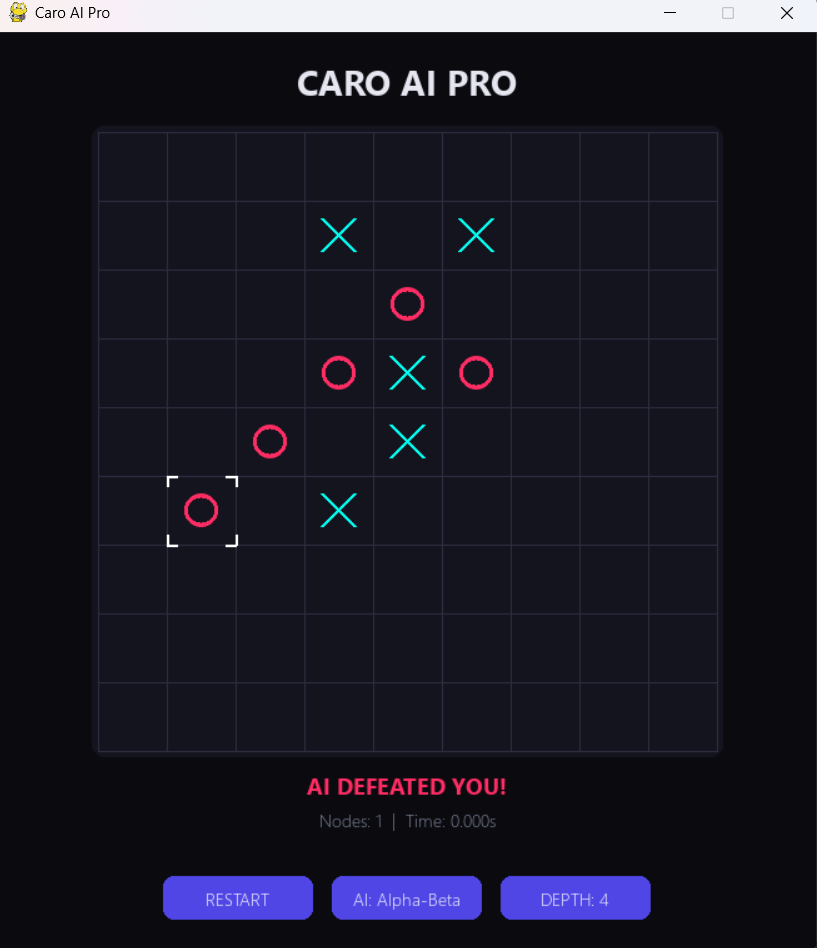
\includegraphics[width=0.7\textwidth]{image/B.png}
    \caption{Giao diện người dùng (UI) cờ Caro trong quá trình chơi}
    \label{fig:ui_demo}
\end{figure}

\subsection{Hạn chế và Hướng phát triển}
\begin{itemize}
    \item \textbf{Hạn chế:} Chưa tích hợp Cơ sở dữ liệu Khai cuộc (Opening Book), dẫn đến việc thuật toán có thể mất thời gian không cần thiết ở những lượt đi đầu tiên. Hàm lượng giá hiện tại chủ yếu phân tích cục bộ thay vì đánh giá toàn cục bàn cờ.
    \item \textbf{Hướng cải tiến:} Tích hợp Zobrist Hashing và hoàn thiện Iterative Deepening để tối ưu việc ghi nhớ trạng thái, từ đó nâng giới hạn độ sâu tìm kiếm lên mức cao hơn ($D \ge 6$).
\end{itemize}

\subsection{Link Repository Github}
Mã nguồn đồ án được quản lý phiên bản trên GitHub tại địa chỉ: \\
\url{https://github.com/tuansonuet197/23021335_23021359_23021273_CaroAI}

\newpage
\section*{Tài liệu tham khảo}
\addcontentsline{toc}{section}{Tài liệu tham khảo}
[1] Bài giảng trên lớp, \textit{Lý thuyết cây trò chơi đối kháng và Giải thuật Alpha-Beta Pruning}. \\
[2] Tài nguyên GitHub mở: \url{https://github.com/husus/gomokuAI-py}. (Nguồn tham khảo cấu trúc thư mục và cách khởi tạo môi trường đồ họa Pygame). \\
[3] Tài nguyên GitHub mở: \url{https://github.com/MonHauVD/Caro_AI}. (Nguồn tham khảo kịch bản đo lường hiệu năng Benchmark). \\

\textit{Lưu ý: Toàn bộ quá trình tư duy logic (Heuristic), xử lý mảng bàn cờ, sinh nước đi và thuật toán đệ quy lõi đều do nhóm tự phân tích thiết kế, dựa trên quy chuẩn luật cờ Caro 4 quân.}

\end{document}
